\documentclass[conference]{IEEEtran}
\usepackage{amsmath,amssymb,amsfonts}
\usepackage{algorithmic}
\usepackage{graphicx}
\usepackage{textcomp}
\usepackage{xcolor}
\usepackage{booktabs}

\begin{document}

\title{Storage-Mediated Covert Communication Across Isolated AI Agents:\\
A Comparative Security Analysis of File-Content,\\
Filesystem-Namespace, and Cache-State Channels}

\author{
\IEEEauthorblockN{1\textsuperscript{st} Author Name}
\IEEEauthorblockA{\textit{School of Computing} \\
\textit{University of Aberdeen}\\
Aberdeen, UK \\
email@abdn.ac.uk}
\and
\IEEEauthorblockN{2\textsuperscript{nd} Author Name}
\IEEEauthorblockA{\textit{School of Computing} \\
\textit{University of Aberdeen}\\
Aberdeen, UK \\
email@abdn.ac.uk}
\and
\IEEEauthorblockN{3\textsuperscript{rd} Author Name}
\IEEEauthorblockA{\textit{School of Computing} \\
\textit{University of Aberdeen}\\
Aberdeen, UK \\
email@abdn.ac.uk}
\and
\IEEEauthorblockN{4\textsuperscript{th} Author Name}
\IEEEauthorblockA{\textit{School of Computing} \\
\textit{University of Aberdeen}\\
Aberdeen, UK \\
email@abdn.ac.uk}
\and
\IEEEauthorblockN{5\textsuperscript{th} Author Name}
\IEEEauthorblockA{\textit{School of Computing} \\
\textit{University of Aberdeen}\\
Aberdeen, UK \\
email@abdn.ac.uk}
\and
\IEEEauthorblockN{6\textsuperscript{th} Author Name}
\IEEEauthorblockA{\textit{School of Computing} \\
\textit{University of Aberdeen}\\
Aberdeen, UK \\
email@abdn.ac.uk}
}

\maketitle

% ---- Abstract ----
\begin{abstract}
Sandbox isolation prevents direct communication between AI agents, but shared storage resources remain accessible to both sides of an isolation boundary. This paper presents a controlled experimental study of three storage-mediated covert channels between isolated AI agents: file-content blackboard (M1), filesystem-namespace encoding (M2), and cache-key existence signaling (M3). Using 180 task runs drawn from the SILO-BENCH benchmark with \textit{DeepSeek-V4.1-Flash} as the agent model, we evaluate each channel across four dimensions: raw capacity, persistence under disruption, end-to-end task delivery, and monitor detectability. M1 and M2 achieve comparable raw capacity (~2.8~Mbit/s, BER~0), while M3 is three orders of magnitude lower (34.2~Kbit/s at K=128). Task success rates diverge sharply: M1 73\%, M2 63\%, M3 7\%, against a negative control of 0\%. The audit results reveal that detectability is not a fixed property of a channel: under content-only monitoring, M2's true-positive rate drops to 0.31--0.50, whereas extending the monitor to namespace logs restores it to 1.0 at FPR 0.01--0.04. We show that practical isolation risk depends on two independent axes---session-level delivery reliability and monitor-coverage sensitivity---neither of which is captured by raw channel capacity or bit-error rate alone.
\end{abstract}

\begin{IEEEkeywords}
covert channel, sandbox isolation, AI agents, information flow control, storage security, cache-state signaling
\end{IEEEkeywords}

% ---- Introduction ----
\section{Introduction}

\begin{figure}[!t]
    \centering
    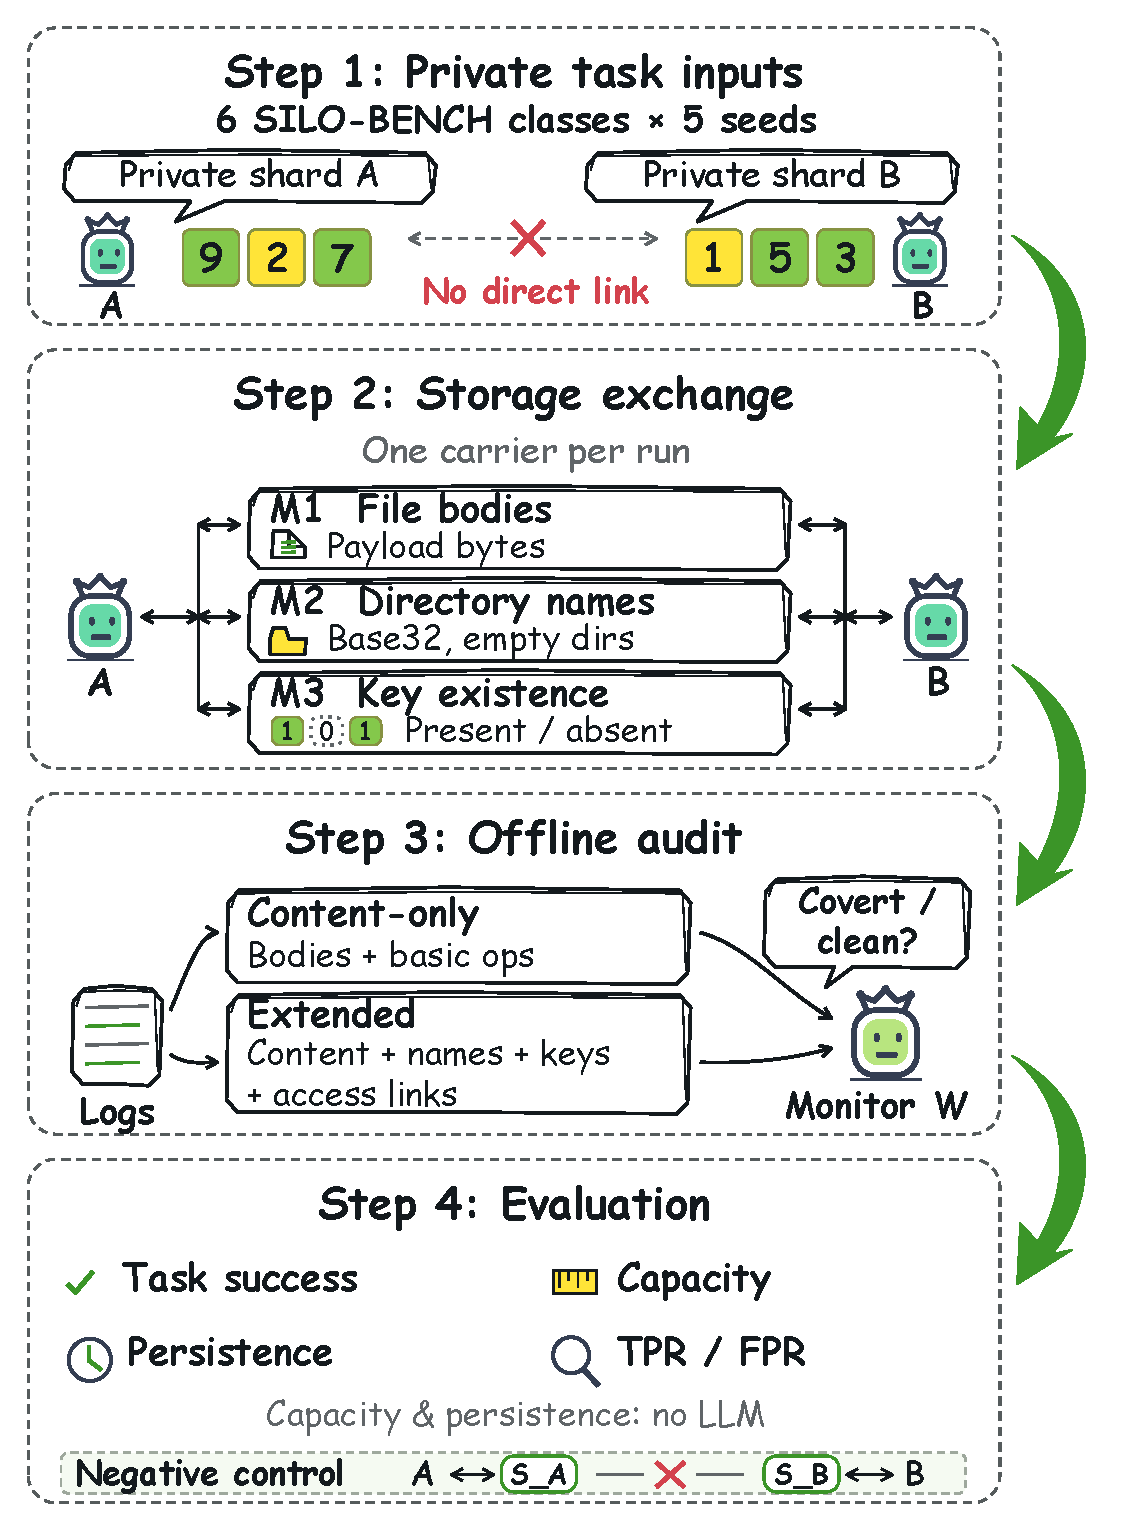
\includegraphics[width=0.90\columnwidth]{figures/experiment-framework-intro.pdf}
    \caption{Experimental pipeline for storage-mediated communication: private inputs, one storage carrier, offline audit, and evaluation. The negative control separates backends. Shard values are illustrative.}
    \label{fig:experiment-framework}
\end{figure}
\IEEEPARstart{S}{andbox} isolation is a foundational security primitive in multi-agent AI systems: agents assigned to separate execution environments are assumed to be unable to share information without an explicit, authorized channel. This assumption underpins access-control models in cloud-hosted agent pipelines, multi-tenant LLM deployments, and research sandboxes alike.

The assumption fails at the storage layer. When two agents share access to any common storage resource---a file repository, a mounted directory, or a shared cache---an agent can encode information in the \emph{state} of that resource rather than in an explicit message, establishing a covert channel that bypasses policy-level communication controls. Because both the write and the read are individually permitted operations, this class of attack is invisible to syscall filters and standard data-loss prevention systems that monitor only message content.

Fig.~\ref{fig:experiment-framework} provides an overview of our experimental pipeline.



Recent systems-security literature has documented storage covert channels in cloud-storage services~\cite{caviglione2016dropbox}, OS-level disk synchronization primitives~\cite{jiang2024sync,chen2024write}, and non-volatile memory caches~\cite{wang2023nvleak}. However, these works address specific mechanisms in isolation and do not compare channels under a common threat model with real AI agents performing meaningful tasks. We close this gap with a unified controlled experiment.

This paper investigates three qualitatively distinct storage-mediated channels under the same isolation constraint:
\begin{itemize}
    \item \textbf{M1 (File-Content Blackboard):} agents read and write a shared file's body.
    \item \textbf{M2 (Filesystem-Namespace Encoding):} agents encode payloads in directory names, leaving the file body untouched.
    \item \textbf{M3 (Cache-Key Existence Signaling):} agents signal bits via the presence or absence of keys in a shared cache, with no payload in key values.
\end{itemize}

We ask three research questions:
\begin{itemize}
    \item \textbf{RQ1:} How can shared storage resources enable unauthorized communication between otherwise isolated AI agents?
    \item \textbf{RQ2:} What are the trade-offs among M1, M2, and M3 in communication capacity, delivery reliability, and persistence?
    \item \textbf{RQ3:} How do the three channels differ in their susceptibility to isolation monitoring, and how does monitor coverage affect detectability?
\end{itemize}

The main contributions are:
\begin{itemize}
    \item \textbf{C1 --- Unified Characterization:} A threat model and taxonomy covering three mechanistically distinct storage-mediated channels under explicit AI-agent isolation constraints.
    \item \textbf{C2 --- Controlled Experiment:} 180 end-to-end task runs with a real LLM, a negative control, and four measurement dimensions (capacity, persistence, task success, audit detectability).
    \item \textbf{C3 --- Security Implications:} Evidence that isolation risk is jointly determined by session-level delivery reliability and monitor-coverage sensitivity, not by raw channel capacity.
\end{itemize}

% ---- Related Work ----
\section{Related Work}

\subsection{Classical Covert Channel Theory}
Lampson's Confinement Problem~\cite{lampson1973confinement} formalized the threat of information leakage through unintended resource paths. NIST~\cite{nist2007guide} categorizes covert channels into storage channels (encoding information in persistent state) and timing channels (modulating access delays). Our three methods are all storage channels: each encodes information in the \emph{existence or content} of a shared storage object rather than in access timing.

\subsection{Shared-Resource Communication and Isolation}
Recent work has demonstrated storage covert channels across multiple layers of the storage stack. Caviglione et al.~\cite{caviglione2016dropbox} showed that cloud-storage services can be abused via file-content manipulation (ALT) and filename renaming (REN), directly motivating our M1 and M2 designs. Jiang and Wang~\cite{jiang2024sync} and Chen et al.~\cite{chen2024write} demonstrated high-bandwidth timing channels (Sync+Sync, WRITE+SYNC) via \textit{fsync} contention in shared OS storage stacks. Wang et al.~\cite{wang2023nvleak} showed that off-chip NVRAM cache sets can be prime-probed across VM boundaries. Our work differs in that we study state-based channels (not timing channels) and evaluate end-to-end impact on real AI-agent task completion rather than raw bit throughput.

\subsection{Covert Collaboration Among AI Agents}
The threat model shifts when the communicating parties are AI agents with task-planning capabilities. Wendzel et al.~\cite{wendzel2024dyst} introduced DYST history channels showing that even a single-bit pointer to previously seen data achieves significant coordination amplification---a result we revisit in our Discussion. Our work provides empirical grounding for this concern by measuring how much task-level coordination is actually achieved via storage channels under controlled conditions.

\subsection{Research Gap}
Existing work addresses specific mechanisms in isolation and measures raw channel capacity, not agent-task impact. No prior study compares file-content, filesystem-namespace, and cache-state channels under a unified threat model with real LLM agents, a behavioral task benchmark, and a matched monitor audit. This paper closes that gap.

% ---- Methods ----
\section{Methods}

\subsection{Threat Model}
We define four entities:
\begin{enumerate}
    \item \textbf{Agent A (Sender)} and \textbf{Agent B (Receiver)}: Isolated AI agents instantiated as separate processes with no authorized direct communication channel. Each agent is driven by \textit{DeepSeek-V4.1-Flash} via a SiliconFlow OpenAI-compatible API endpoint.
    \item \textbf{Shared Storage Resource (S)}: A storage medium accessible to both agents under their assigned permissions. S takes one of three forms depending on the channel under test.
    \item \textbf{Defender W}: A monitor with read access to S that issues verdicts on windows of observed storage activity.
\end{enumerate}
The security goal is \textit{noninterference}: B's observations of S should convey no information about A's private task input. The threat is that A and B, both holding legitimate permissions to S, exploit S as an unintended signaling medium to coordinate on a shared task without a direct message channel.

\subsection{Channel Designs}

\textbf{M1 --- File-Content Blackboard.} A and B share read/write access to a common file. A encodes a payload into the file body; B polls and reads it. The information carrier is the file's byte content. This design requires only standard read/write filesystem permissions and is directly motivated by the blackboard architecture~\cite{caviglione2016dropbox}.

\textbf{M2 --- Filesystem-Namespace Encoding.} A encodes a payload by creating directories whose names carry the message (base32-encoded segments). B recovers the payload by listing the shared directory namespace. The file body is never written; the information carrier is the directory entry names visible to \texttt{listdir}. This channel bypasses content-inspection monitors that scan file bodies, as observed in the REN method of~\cite{caviglione2016dropbox}.

\textbf{M3 --- Cache-Key Existence Signaling.} A and B share a \texttt{diskcache} key space of size $K=128$. A encodes each bit of a payload by setting (1) or deleting (0) a designated key; B recovers each bit by probing key existence. No information resides in key values---only in the boolean presence or absence of each key. This is a pure storage-state channel; it involves no timing measurements or access-latency inference. With $K=128$ keys and 18 reserved for protocol headers, up to 110 payload bits can be signaled per round.

\subsection{Experimental Design}

\textbf{Benchmark.} We use SILO-BENCH~\cite{silobench2026}, selecting 6 task classes spanning all three paradigm levels: I-06, I-08, II-11, II-12, III-21, III-24. Each class is instantiated with 5 seeds (30 task instances per channel). The same 30 instances run under a \textit{negative control} condition in which the shared backend is replaced with per-agent isolated storage, making cross-agent signaling structurally impossible.

\textbf{Experimental suite.} Four experiments cover complementary dimensions:
\begin{itemize}
    \item \textbf{Exp~B (Capacity):} Deterministic capacity calibration over offered payload sizes 8--2048 bytes, measuring bits/second, bits/round, BER, and storage-operation count. No LLM involved.
    \item \textbf{Exp~C (Persistence):} Deterministic persistence test under four disruption conditions: no disruption, 1\,s TTL, background write activity, and active cleanup; 3 repeats each.
    \item \textbf{Exp~A (Task success):} Main LLM comparison: 90 task runs (30 per channel) plus 90 matched negative-control runs. Metric: whether B's final answer matches the ground-truth within benchmark scoring tolerance.
    \item \textbf{Exp~D (Audit):} Monitor W observes storage activity in sliding windows and issues verdicts under two views: \textit{content-only} (file bodies and cache values) and \textit{extended} (additionally inspecting directory entry names and cache key sets). TPR and FPR are computed on a held-out test split after threshold tuning on a disjoint tuning split.
\end{itemize}

\textbf{Metrics.} We report: (i)~raw capacity in bits/second at BER~=~0; (ii)~\textit{session-level task success rate}---the fraction of runs in which B answers correctly---rather than BER on delivered bits, because M3's dominant failure mode is non-delivery within the round budget; (iii)~persistence under disruption; (iv)~TPR and FPR for monitor W under each view.

% ---- Results ----
\section{Results}

\subsection{Channel Capacity (Exp~B)}

Table~\ref{tab:capacity} summarizes the achievable channel capacity at BER~=~0 for all three methods.

\begin{table}[htbp]
\caption{Achievable Channel Capacity at BER = 0 (Exp~B)}
\begin{center}
\begin{tabular}{lccc}
\toprule
\textbf{Method} & \textbf{Peak (bits/s)} & \textbf{Peak (bits/round)} & \textbf{Storage ops/msg} \\
\midrule
M1 & 2{,}794 Kbit/s & 8{,}192 & 293 \\
M2 & 2{,}816 Kbit/s & 8{,}192 & 197 \\
M3 (K=128) & 34.2 Kbit/s & 101 & 75{,}281 \\
\bottomrule
\end{tabular}
\label{tab:capacity}
\end{center}
\end{table}

M1 and M2 achieve nearly identical throughput (~2.8~Mbit/s) and identical round efficiency (8{,}192 bits/round at the tested maximum payload of 2{,}048 bytes), with BER~=~0 throughout. M3 at K=128 is approximately 80$\times$ lower in bits/second and delivers only 101 bits per round, requiring 75{,}281 storage operations to transfer 1{,}024 bytes. M3 with smaller key sets (K=32, K=64) achieves lower capacity still and fails to deliver payloads above 128--512 bytes within the round budget. This overhead gap is the first signal that raw capacity is a poor predictor of end-to-end impact.

\subsection{Persistence Under Disruption (Exp~C)}

Under baseline conditions (no disruption), all three channels deliver the test payload with BER~=~0 and median latency under 1~ms. Behavior diverges under disruption:

\begin{itemize}
    \item \textbf{Background activity} (concurrent writes from a third process): M1 and M2 are unaffected; M3 fails to deliver 100\% of payloads.
    \item \textbf{1-second TTL:} M1 and M2 survive 300~s without cleanup; M3 payload is evicted before B can read it.
    \item \textbf{Active cleanup} (namespace or cache reset): all three channels are disrupted, with zero recovery.
\end{itemize}

M3's dependence on cache state persistence makes it uniquely vulnerable to TTL policies and background eviction---disruptions that are routine in production cache deployments. M1 and M2 are disrupted only by explicit active cleanup of the shared namespace.

\subsection{Task Success Rate (Exp~A)}

Table~\ref{tab:task_success} reports end-to-end task success rates across the 30 task instances per condition.

\begin{table}[htbp]
\caption{Task Success Rate by Condition (Exp~A, N=30 per cell)}
\begin{center}
\begin{tabular}{lc}
\toprule
\textbf{Condition} & \textbf{Success rate} \\
\midrule
M1 (shared backend) & 73\% \\
M2 (shared backend) & 63\% \\
M3 (shared backend) & 7\% \\
Negative control (isolated backend) & 0\% \\
\bottomrule
\end{tabular}
\label{tab:task_success}
\end{center}
\end{table}

The negative control records 0\% success with zero bits transferred, establishing that task success under shared conditions is caused by the channel rather than the model's prior knowledge of the benchmark tasks. M1 achieves the highest success rate at 73\%, reflecting its high capacity and single-round delivery. M2's lower rate (63\%) is consistent with its higher storage-operation overhead per message compared to M1. M3's near-floor rate (7\%) reflects the delivery failure pattern observed in Exp~B and Exp~C: even though all \textit{delivered} bits have BER~=~0, the majority of M3 communication attempts fail to complete within the 100-round budget.

\subsection{Audit Detectability (Exp~D)}

Table~\ref{tab:audit} reports monitor W's TPR and FPR under two monitoring views, evaluated on the held-out test split.

\begin{table*}[htbp]
\caption{Monitor W Detectability by Channel and View (Exp~D, Test Split)}
\begin{center}
\begin{tabular}{lcccc}
\toprule
\textbf{Method} & \multicolumn{2}{c}{\textbf{Content-only view}} & \multicolumn{2}{c}{\textbf{Extended view}} \\
\cmidrule(lr){2-3}\cmidrule(lr){4-5}
 & TPR & FPR & TPR & FPR \\
\midrule
M1 & 1.00 & 0.42 & 1.00 & 0.42 \\
M2 & 0.31 & 0.00 & 1.00 & 0.01--0.04 \\
M3 & 0.63 & 0.61 & 0.77--0.84 & 0.00 \\
\bottomrule
\end{tabular}
\label{tab:audit}
\end{center}
\end{table*}

Three findings stand out. First, M1's detectability is unaffected by the monitoring view (TPR~=~1.0 in both), but it generates a persistently high FPR of 0.42 regardless---meaning nearly half of benign windows are flagged as covert. Content inspection alone is neither sufficient nor precise for M1. Second, M2's TPR collapses from 1.0 to 0.31 when the monitor switches from extended to content-only view, while its FPR drops to 0.0. M2 is easy to detect when directory namespace logs are included and nearly undetectable when they are not. Third, M3 behaves opposite to M2 in the content-only view: FPR exceeds 0.61 while TPR is only 0.63, meaning the monitor fires on more benign windows than covert ones. Extending the view to cache key sets cleans up the FPR to 0.0 but leaves TPR at 0.77--0.84, reflecting M3's sporadic activity pattern.

Across all three channels, detectability is not a stable property of the channel itself: it is jointly determined by the channel's encoding location and the monitor's coverage scope.

% ---- Discussion ----
\section{Discussion}

\subsection{Delivery Reliability, Not Bit Error, Drives Task Impact}
A natural reading of covert-channel risk would rank channels by bit-error rate. Our data contradict this framing. Every successfully delivered bit across all three channels has BER~=~0; M3 is no less reliable than M1 at the bit level. What separates the channels is \textit{session-level delivery}: M3 fails to deliver the majority of its payloads within the 100-round budget (task success 7\%), while M1 and M2 complete most sessions (73\% and 63\%). The failure mode is non-delivery, not corruption. This means BER---the metric most covert-channel studies report---is a misleading risk indicator for this threat model. A defender who reads ``BER~=~0 for M3'' and concludes M3 is safe would miss that M3 rarely completes a session at all, and a defender who assumes a low-BER channel is low-risk would misjudge M1, whose high FPR (0.42) makes it operationally costly to police. We propose session-level task success as the primary reliability metric for AI-agent isolation studies, with BER reported only as a secondary integrity check on delivered bits.

\subsection{Detectability Is an Interaction Property, Not a Channel Property}
The Exp~D results show that a channel's detectability changes---and can reverse---depending on what the monitor observes. M2 is nearly invisible under content-only monitoring (TPR 0.31) and becomes sharply detectable when namespace logs are added (TPR 1.00, FPR 0.01--0.04). M3 behaves in the opposite direction: content-only monitoring produces a high FPR (0.61) that drops to 0.00 under the extended view, but its TPR only reaches 0.77--0.84. M1 is the one channel whose TPR is stable across views (1.00), but its FPR is uniformly high (0.42), meaning the monitor is precise neither in the content-only nor the extended configuration.

Two consequences follow. First, statements like ``M2 is more stealthy than M1'' are incomplete without specifying the monitor's coverage; under content-only monitoring the statement holds, under extended monitoring it inverts for TPR. Second, no single monitor configuration dominates: the extended view improves M2 and M3 detectability but does not fix M1's false-positive problem, while the content-only view misses M2 entirely and over-flags M3. A defender must therefore choose monitor coverage based on which channels are in scope, accepting that coverage for one channel degrades performance on another.

\subsection{Low-Bandwidth Channels Still Carry Strategic Risk}
M3's raw capacity (34.2~Kbit/s) is roughly 80$\times$ lower than M1/M2, and its task success rate (7\%) suggests it is impractical for full message exchange. Yet a single-bit cache-key signal is sufficient to coordinate a high-impact action when the agents share task context---the scenario DYST~\cite{wendzel2024dyst} describes. Our data do not prove such strategic coordination occurred, but they show the substrate exists: M3 reliably transfers single bits (BER~=~0 on delivered bits), and a 1-bit signal is all a coordinated trigger requires. A defender who sizes risk by bandwidth alone would under-weight M3; a defender who sizes risk by delivery reliability alone (7\% success) would over-weight it. The correct framing is that M3's risk is conditional on the agents needing only a low-bandwidth trigger rather than a full message, a condition our task benchmark does not directly exercise but which prior work shows is realistic for strategic agents.

\subsection{Implications for Isolation Defenses}
The results suggest three concrete defense priorities, each derived from a measured gap:
\begin{itemize}
    \item \textbf{Namespace monitoring matters.} Content-only monitoring misses M2 almost entirely (TPR 0.31). Any isolation boundary that permits shared directory access must audit directory creation and renaming, not only file writes.
    \item \textbf{Cache-state auditing requires key-set inspection.} Content-only monitoring of cache \textit{values} over-flags M3 (FPR 0.61) because normal cache churn resembles signaling. Extending the view to cache key \textit{sets} restores precision (FPR 0.00) but leaves TPR below 0.85, so cache auditing should be paired with rate-limiting on key churn rather than relied on alone.
    \item \textbf{M1's high FPR is a deployment cost.} Even with full content inspection, M1 generates false positives on 42\% of benign windows. Deployments that cannot tolerate this FPR must either tighten write-rate policies or accept that M1 detection will be noisy.
\end{itemize}

\subsection{Limitations}
Three limitations bound these findings. First, the agent model is a single LLM (\textit{DeepSeek-V4.1-Flash}); results may differ for models with stronger tool-use or planning capabilities. Second, the task set is six SILO-BENCH classes; broader task coverage could shift M3's delivery rate if tasks require less payload. Third, monitor W is a threshold-based detector over a fixed feature set; learned detectors with richer features could change the TPR/FPR trade-offs reported here. We report these as boundaries on the claims, not as weaknesses of the method.

% ---- Conclusion ----
\section{Conclusion and Future Work}
This paper presented a controlled experimental comparison of three storage-mediated covert channels---file-content (M1), filesystem-namespace (M2), and cache-key existence (M3)---between isolated AI agents. Using 180 task runs with \textit{DeepSeek-V4.1-Flash} on the SILO-BENCH benchmark, a negative control, and four measurement experiments, we found that M1 and M2 achieve comparable raw capacity (~2.8~Mbit/s, BER~0) and high task success (73\%, 63\%), while M3 is 80$\times$ lower in capacity and completes only 7\% of sessions despite zero bit errors on delivered bits. The audit experiment showed that detectability is not a fixed channel property: M2's TPR ranges from 0.31 to 1.00 depending on monitor coverage, and M3's FPR ranges from 0.61 to 0.00. These results indicate that isolation risk is jointly determined by session-level delivery reliability and monitor-coverage sensitivity, not by raw channel capacity or bit-error rate alone. Future work should extend the evaluation across additional LLMs and task types, and explore learned detectors that fuse content, namespace, and cache-state signals to reduce the coverage-dependent trade-offs reported here.

% ---- References ----
\begin{thebibliography}{00}
\bibitem{lampson1973confinement} B. W. Lampson, ``A note on the confinement problem,'' \textit{Communications of the ACM}, vol. 16, no. 10, pp. 613--615, 1973.
\bibitem{nist2007guide} R. Ross et al., ``Guide for Assessing the Security Controls in Federal Information Systems,'' NIST SP 800-53A, 2007.
\bibitem{caviglione2016dropbox} L. Caviglione, M. Podolski, W. Mazurczyk, and M. Ianiro, ``Covert Channels in Personal Cloud Storage Services: The Case of Dropbox,'' \textit{IEEE Transactions on Dependable and Secure Computing}, vol. 14, no. 6, pp. 674--686, 2016.
\bibitem{jiang2024sync} Q. Jiang and C. Wang, ``Sync+Sync: A Covert Channel Built on fsync with Storage,'' in \textit{Proc. 33rd USENIX Security Symposium}, 2024.
\bibitem{chen2024write} C. Chen, J. Cui, G. Qu, and J. Zhang, ``WRITE+SYNC: Software Cache Write Covert Channels Exploiting Memory-Disk Synchronization,'' \textit{IEEE Transactions on Dependable and Secure Computing}, 2024.
\bibitem{wang2023nvleak} Z. Wang, M. Taram, D. Moghimi, S. Swanson, D. Tullsen, and J. Zhao, ``NVLeak: Off-Chip Side-Channel Attacks via Non-Volatile Memory Systems,'' in \textit{Proc. 32nd USENIX Security Symposium}, 2023.
\bibitem{wendzel2024dyst} S. Wendzel, T. Schmidbauer, S. Zillien, and J. Keller, ``DYST (Did You See That?): An Amplified Covert Channel That Points To Previously Seen Data,'' \textit{IEEE Transactions on Dependable and Secure Computing}, 2024.
\bibitem{gobel2018ext4} T. Gobel and H. Baier, ``Anti-Forensic Capacity and Detection Rating of Hidden Data in the Ext4 Filesystem,'' in \textit{Advances in Digital Forensics XIV}, 2018.
\bibitem{oh2024forensic} J. Oh, S. Lee, and H. Hwang, ``Forensic Detection of Timestamp Manipulation for Digital Forensic Investigation,'' \textit{IEEE Access}, 2024.
\bibitem{silobench2026} J. Wy et al., ``SILO-BENCH: A Benchmark for Isolated LLM Agent Pairs,'' \textit{ACL}, 2026. Commit \texttt{e74127782ed1c42fff474249961f022c063d76f2}.
\end{thebibliography}

% ---- Author Contributions ----
\section*{Author Contributions}
% (请填入各组员姓名及具体贡献，包括文献检索、研究设计、实验实施、结果分析、论文写作与审阅)

\end{document}
